\documentclass[12pt]{ctexart}
    %%% Document Settings %%%%
%\usepackage[utf8]{inputenc}

\usepackage[
    twoside,
    top=1in,
    bottom=0.75in,
    inner=0.5in,
    outer=0.5in,
]{geometry}
\pagestyle{myheadings}
\usepackage[dvipsnames,svgnames]{xcolor}

%%%% Additional Commands to Load %%%%
\usepackage{tcolorbox}
\tcbuselibrary{skins}
%\usepackage{minted}
\usepackage{color}
\usepackage{tikz}
\usetikzlibrary{calc}
\usepackage{tabularx,colortbl}
\usepackage{amsfonts,amsmath,amssymb}
\usepackage{titling}
\usepackage{mathrsfs}
\usepackage{calc}
\usepackage{subcaption}

\usepackage{listings}
%\usepackage{newtxtext}
\usepackage[strict]{changepage} 
\usepackage{framed}
\definecolor{formalshade}{rgb}{0.95,0.95,1}

%%%% Commands to Define Homework Boxes %%%%
%%%% Box Definition %%%%
\newtcolorbox{prob}[1]{
% Set box style
    sidebyside,
    sidebyside align=top,
% Dimensions and layout
    width=\textwidth,
    toptitle=2.5pt,
    bottomtitle=2.5pt,
    righthand width=0.20\textwidth,
% Coloring
    colbacktitle=gray!30,
    coltitle=black,
    colback=white,
    colframe=black,
% Title formatting
    title={
        #1 \hfill Grade:\phantom{WWWW}
    },
    fonttitle=\large\bfseries
}

%%%% Environment Definition %%%%
\newenvironment{problem}[1]{
    \begin{prob}{#1}
}
{
    \tcblower
    \centering
    \textit{\scriptsize\bfseries Faculty Comments}
    \vspace{\baselineskip}
    \end{prob}
}

\newenvironment{formal}{%
\def\FrameCommand{%
\hspace{1pt}%
{\color{DarkBlue}\vrule width 2pt}%
{\color{formalshade}\vrule width 4pt}%
\colorbox{formalshade}%
}%
\MakeFramed{\advance\hsize-\width\FrameRestore}%
\noindent\hspace{-4.55pt}% disable indenting first paragraph
\begin{adjustwidth}{}{7pt}%
\vspace{2pt}\vspace{2pt}%
}
{%
\vspace{2pt}\end{adjustwidth}\endMakeFramed%
}

    \title{课后作业:一维模型大地电磁响应的差分解法}
    \author{杨曜堃\ 张浩宇}
    \date{\today}
%%% document
\begin{document}

% Format Running Header
    \markboth{\theauthor}{\thetitle}
    \maketitle
    \subsection*{1\ \ \ 差分正演算法推导}
    一维大地介质中,电场满足微分方程
    \begin{equation}
        \dfrac{\partial^2E_x}{\partial z^2}+i\omega\mu\sigma(z)E_x=0\label{1} 
    \end{equation}

    其中$\sigma$为介质的电导率,其单位为$\mathrm{S/m}$,$\mu$为介质的磁导率,取$\mu=4\pi\times10^{-7}\mathrm{H/m}$。

    使用有限差分法求解,对电场离散化,如图\ref{fig1}所示
    \begin{figure}[htbp]
        \small
        \centering
        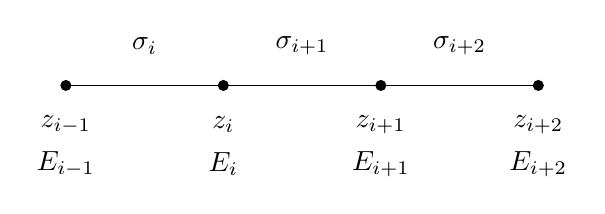
\begin{tikzpicture}
            \coordinate[] (A) at (0,0);
            \coordinate[] (B) at (2,0);
            \coordinate[] (C) at (4,0);
            \coordinate[] (D) at (6,0);
            \fill[] (A)circle(2pt);
            \fill[] (B)circle(2pt);
            \fill[] (C)circle(2pt);
            \fill[] (D)circle(2pt);
            \draw[] (A)--(B);
            \draw[] (B)--(C);
            \draw[] (C)--(D);
            \node[] (a) at (0,-0.5) {$z_{i-1}$};
            \node[] (b) at (2,-0.5) {$z_{i}$};
            \node[] (c) at (4,-0.5) {$z_{i+1}$};
            \node[] (d) at (6,-0.5) {$z_{i+2}$};
            \node[] (e) at (0,-1) {$E_{i-1}$};
            \node[] (f) at (2,-1) {$E_{i}$};
            \node[] (g) at (4,-1) {$E_{i+1}$};
            \node[] (h) at (6,-1) {$E_{i+2}$};
            \node[] (i) at (1,0.5) {$\sigma_{i}$};
            \node[] (j) at (3,0.5) {$\sigma_{i+1}$};
            \node[] (k) at (5,0.5) {$\sigma_{i+2}$};
        \end{tikzpicture}
        \caption{电场离散化} \label{fig1}
    \end{figure}

    采用有限差分法计算偏导数
    \begin{equation}
        \left.\dfrac{\partial^2E}{\partial z^2}\right|_{z_i}=\dfrac{1}{\Delta z^2}\left(E_{i-1}-2E_{i}+E_{i+1}\right)\label{2}
    \end{equation}

    将式\eqref{2}代入式\eqref{1}可得
    \begin{equation}
        \dfrac{1}{\Delta z^2}(E_{i-1}-2E_i+E_{i+1})+i\omega\mu\left(\dfrac{\sigma_i+\sigma_{i+1}}{2}\right)E_i=0\label{3}
    \end{equation}

    即
    \begin{equation}
        \dfrac{1}{\Delta z^2}E_{i-1}+\left[i\omega\mu\left(\dfrac{\sigma_{i}+\sigma_{i+1}}{2}\right)-\dfrac{2}{\Delta z^2}\right]E_i+\dfrac{1}{\Delta z^2}E_{i+1}=0
        \label{4}
    \end{equation}

    将式\eqref{4}推广到所有节点,并写成矩阵形式
    \begin{equation}
        \begin{bmatrix}
            \frac{1}{\Delta z^2} & i\omega\mu\left(\frac{\sigma_{1}+\sigma_2}{2}\right)-\frac{2}{\Delta z^2} & \frac{1}{\Delta z^2} & 0 & \cdots & 0 \\
            0 & \frac{1}{\Delta z^2} & i\omega\mu\left(\frac{\sigma_{2}+\sigma_3}{2}\right)-\frac{2}{\Delta z^2} & \frac{1}{\Delta z^2} & \cdots & 0 \\
            \vdots & \vdots & \ddots & \ddots & \ddots & \vdots \\
            0 & 0 & \cdots & \frac{1}{\Delta z^2} & i\omega\mu\left(\frac{\sigma_{N-1}+\sigma_N}{2}\right)-\frac{2}{\Delta z^2} & \frac{1}{\Delta z^2}
        \end{bmatrix}
        \begin{bmatrix}
            E_1 \\
            E_2 \\
            \vdots \\
            E_{N-1}
        \end{bmatrix}=
        \begin{bmatrix}
            0 \\
            0 \\
            \vdots \\
            0
        \end{bmatrix}
        \label{5}
    \end{equation}

    为了使方程组可解,需加入边界条件。由上边界条件,电场在空气中不衰减,取$E_0=1$。对于下边界,电磁波按复指数衰减,因而满足微分方程
    \begin{equation}
        \dfrac{\partial E_x}{\partial z}+kE_x=0\label{6}
    \end{equation}

    将式\eqref{6}转为差分格式
    \begin{equation}
        \left(\dfrac{1}{\Delta z}+k\right)E_N-\dfrac{1}{\Delta z}E_{N-1}=0\label{7}
    \end{equation}

    将边界条件加入式\eqref{5},可得完整线性方程组
    \begin{formal}
        \begin{equation*}
            \begin{bmatrix}
                1 & 0 & 0 & 0 & \cdots & 0 \\
                \frac{1}{\Delta z^2} & i\omega\mu\left(\frac{\sigma_{1}+\sigma_2}{2}\right)-\frac{2}{\Delta z^2} & \frac{1}{\Delta z^2} & 0 & \cdots & 0 \\
                0 & \frac{1}{\Delta z^2} & i\omega\mu\left(\frac{\sigma_{2}+\sigma_3}{2}\right)-\frac{2}{\Delta z^2} & \frac{1}{\Delta z^2} & \cdots & 0 \\
                \vdots & \vdots & \ddots & \ddots & \ddots & \vdots \\
                0 & 0 & \cdots & \frac{1}{\Delta z^2} & i\omega\mu\left(\frac{\sigma_{N-1}+\sigma_N}{2}\right)-\frac{2}{\Delta z^2} & \frac{1}{\Delta z^2}\\
                0 & 0 & \cdots & 0 & -\frac{1}{\Delta z} & \frac{1}{\Delta z}+k
            \end{bmatrix}
            \begin{bmatrix}
                E_0 \\
                E_2 \\
                E_3 \\
                \vdots \\
                E_{N-1} \\
                E_N
            \end{bmatrix}=
            \begin{bmatrix}
                1 \\
                0 \\
                0 \\
                \vdots \\
                0 \\
                0
            \end{bmatrix}
        \end{equation*}
    \end{formal}
    
    从而可以求出$E_x$,进一步可以求出视电阻率和相位
    \begin{subequations}
        \begin{gather}
            Z_{\text{1D}}=E_x\left(\dfrac{1}{i\omega\mu}\dfrac{\partial E_x}{\partial z}\right)^{-1}\label{8a}\\
            \rho_a=\dfrac{1}{\omega \mu}|Z_{ID}|^2\label{8b}\\
            \theta = \mathrm{arctan}\dfrac{\mathrm{Re}\{Z_{\text{1D}}\}}{\mathrm{Im}\{Z_{\text{1D}}\}}\label{8c}
        \end{gather}
    \end{subequations}

    其中$Z_{\mathrm{1D}}$是地表处的阻抗,即地表处电场与磁场之比。为了提高视电阻率计算精度,将偏导数写成
    \begin{equation}
        \left.\dfrac{\partial E_x}{\partial z}\right|_{z=0}=\dfrac{1}{2L}(-11E_0+18E_1-9E_2+2E_3)\label{9}
    \end{equation}

    其中$L$为节点1至节点4的距离。
    \subsection*{2\ \ \ 一维模型试算分析}
    选取二层G型地电模型,其模型参数为$\sigma_1=0.1\mathrm{S/m}$,$\sigma_2=0.01\mathrm{S/m}$,$h=1000\mathrm{m}$,如图\ref{fig2}所示。
    \begin{figure}[H]
        \small
        \centering
        \begin{tikzpicture}
            \draw[->] (0,0)--(8,0);
            \draw[->] (0,0)--(0,-4.4);
            \draw[->] (0,0)--(5,2);
            \draw[] (0,-2)--(8,-2);
            \node[] (O) at (-0.4,0) {$O$};
            \node[] (x) at (5.3,1.8) {$x$};
            \node[] (y) at (8.4,0) {$y$};
            \node[] (z) at (0,-4.7) {$z$};
            \node[] (s1) at (3,-1) {$\sigma_1=0.1\mathrm{S/m}$};
            \node[] (s2) at (3,-3) {$\sigma_2=0.01\mathrm{S/m}$};
            \node[] (h) at (7,-1.6) {$h=1000\mathrm{m}$};
        \end{tikzpicture}
        \caption{二层G型地电模型}\label{fig2}
    \end{figure}

    根据有限差分法正演公式,编写MATLAB程序,计算结果如图\ref{fig3}所示
    \begin{figure}[htbp]
        \small
        \centering
        \includegraphics[width=16cm]{Fig1.png}
        \caption{正演计算结果图} \label{fig3}
    \end{figure}
    % \begin{tcblisting}{listing engine=minted,boxrule=0.1mm,
    %     colback=blue!5!white,colframe=blue!75!black,
    %     listing only,left=5mm,
    %     minted language=matlab,
    %     minted options={fontsize=\small,breaklines, autogobble,linenos,numbersep=3mm}}
        
    % \end{tcblisting}
    % \begin{lstlisting}[language = Matlab,title={test4\_script.m},  numbers=left, 
    %     numberstyle=\tiny,keywordstyle=\color{blue!70},
    %     commentstyle=\color{red!50!green!50!blue!50},frame=shadowbox,
    %     rulesepcolor=\color{red!20!green!20!blue!20},basicstyle=\ttfamily]
    % \end{lstlisting}
\end{document}